\documentclass[journal]{./IEEE/IEEEtran}
\usepackage{cite,graphicx}
\usepackage{makecell}
\usepackage{amsmath}

\newcommand{\SPTITLE}{Using Emotion Word Intensities for Multi-label Emotion Detection of Text}
\newcommand{\ADVISEE}{Andrei Francis U. Enrique}
\newcommand{\ADVISER}{Maria Art Antonette D. Clariño}

\newcommand{\BSCS}{Bachelor of Science in Computer Science}
\newcommand{\ICS}{Institute of Computer Science}
\newcommand{\UPLB}{University of the Philippines Los Ba\~{n}os}
\newcommand{\REMARK}{\thanks{Presented to the Faculty of the \ICS, \UPLB\
                             in partial fulfillment of the requirements
                             for the Degree of \BSCS}}
        
\markboth{CMSC 190 Special Problem, \ICS}{}
\title{\SPTITLE}
\author{\ADVISEE~and~\ADVISER%
\REMARK
}
\IEEEoverridecommandlockouts
% \IEEEpubid{\makebox[\columnwidth]{\copyright~2023~ICS \UPLB \hfill} \hspace{\columnsep}\makebox[\columnwidth]{ }}
\pubid{\copyright~2024~ICS \UPLB}

%%%%%%%%%%%%%%%%%%%%%%%%%%%%%%%%%%%%%%%%%%%%%%%%%%%%%%%%%%%%%%%%%%%%%%%%%%

\begin{document}

% TITLE
\maketitle

% ABSTRACT
\begin{abstract}
Emotion word intensity values were derived from an emotion intensity lexicon and used along with n-grams as baseline features to create a linear support vector machine classifier using the one-vs-rest strategy for multi-labeled emotion data. The model was trained on a dataset of English subtitles and compared to a similarly configured classifier which only included baseline features. The results showed that the classifier with emotion intensity values performed significantly better than the model without these features, achieving a macro f1 score of 0.4359. Furthermore, emotion intensity values for disgust, fear, joy, and sadness showed very high feature importance for their respective emotion labels. The findings suggest that the use of emotion word intensities can help classification models in identifying the emotions expressed within bodies of text.
\end{abstract}

% INDEX TERMS
\begin{keywords}
Sentiment Analysis, Text-based Emotion Detection, Emotion Intensity, NLP, Multi-label Classification
\end{keywords}

% INTRODUCTION
\section{Introduction}
% To be effective, the introduction should answer the questions ``Why and What For (Four)?" Expanded, these questions are:\cite{Papadakis83}

\subsection{Background of the Study}
Emotions play a vital role in human life. They enable us to express our feelings, preferences, and needs to ourselves and others. Emotions can also affect how we assess situations, consider different options, and make decisions\cite{Alzoubi1}. Our emotions are manifested in various ways, such as our speech, our facial expressions, and the words that we write.

Billions of people from around the world use online social platforms to create and share various types of digital content. These platforms contain a wealth of textual data, including forum discussions, blogs, product reviews, and more\cite{Hartmann1}. These platforms may also encourage users to express their thoughts and opinions on specific topics, which can allow people to make observations on how sentiments vary across a range of topics. Because of this, the analysis of emotions and sentiments of people from bodies of text can provide valuable insights for fields such as business and psychology. Hence, text-based emotion detection has become an important area of research.

Emotion analysis has been used in many real-life applications. It is able to provide additional granularity to areas that are traditionally served by polarity-based sentiment analysis\cite{Kusal1}. The emotions derived from a body of text can vary based on the approach that is used. Many existing emotion analysis studies look at the presence of emotion words in bodies of text, and how they relate to other features present in the text. Emotion words are obtained through a lexicon which indicates if a word in the text is associated with one or more emotions. Valuable insight into how emotions influence online behavior and perception has been obtained through this approach, such as in news\cite{Xu1}, e-commerce\cite{Chatterjee1}, and social media\cite{Chung1}.

\subsection{Statement of the Problem}
Though lexicon-based approaches are still popular for applications of emotion analysis, they have been eclipsed in performance by more advanced approaches to emotion detection. Multi-labeled datasets are also becoming more widely available, further increasing the need for a more refined approach to the use of emotion lexicons.

More advanced emotion lexicons have been released that may help mitigate particular shortcomings. Among them is the NRC Emotion Intensity Lexicon\cite{Mohammad2}, which uses best-worst scaling (BWS) to determine the degree to which a word is associated with a particular emotion. This study uses this lexicon alongside other classification features to develop a method for identifying emotions in text.

\subsection{Significance of the Study}

\pubidadjcol This study was useful in developing a better understanding of how to automatically identify the emotions expressed by a body of text. A better understanding of text-based emotion detection can pave the way for future researchers to develop even more accurate and robust emotion detection classifiers, especially those that are able to identify multiple emotions. This can also help future emotion analysis studies that need to automatically determine the emotions expressed by text by providing a model that is more representative of the true emotions of text, as compared to using an emotion lexicon.

\subsection{Objectives of the Study}
\pubidadjcol The general objective of this study is to utilize emotion word intensities to implement a classification model that can identify the emotions expressed by a body of text. The specific objectives are the following:

\begin{itemize}
    \item{Identify the relationship between the presence of emotion words in a body of text and the emotions expressed within said body of text,}
    \item{Determine the importance of emotion word intensities in relation to other features used in classification models to identify the emotions expressed in text,}
    \item{Evaluate the performance of the machine learning model in classifying multi-labeled emotion data using metrics such as per-label F1 score and macro F1 score, and test these metrics against a baseline model for statistical significance.}
\end{itemize}

\subsection{Scope and Limitations of the Study}
This study is limited only to the development and testing of a classification model that uses values obtained from an emotion word lexicon to identify multi-labeled emotion data. The term "emotion words" in the context of this study is only used to refer to words present in the utilized lexicon with intensity values greater than zero. The classification model was trained and tested only using text in the English language. The classification performance of the model was evaluated by comparing the emotion labels it identifies with the true emotion labels of the body of text, as identified by the original annotators of the dataset. The emotion labels used in the classification of text was limited only to the list of emotions present in the dataset, excluding the "neutral" label as this indicates that the dataset does not classify the text under any of the given emotions.

% RRL
\section{Review of Related Literature}
\subsection{Sentiment and Emotion Analysis}
Sentiment analysis is the process of using natural language processing (NLP) and other computational techniques to identify and extract feelings or opinions expressed by a given source\cite{Wankhade1}. Text is by far the most commonly used source, but others include speech, facial expression, body language, and more. Sentiment analysis is generally concerned with identifying the sentiment polarity of a given text, whether it be positive, negative, or neutral. It is a useful technique for applications such as customer feedback, social media analysis, product reviews, and natural language understanding.

Emotion analysis falls under the wider field of sentiment analysis, generally concerned with identifying discrete emotions within a given body of text\cite{Yadollahi1}. This is done with the goal of providing additional granularity to existing applications of sentiment analysis. For example, one may want to differentiate between text that conveys anger to text that conveys sadness, despite both being of negative sentiment. Certain emotion models may also provide labels that do not definitively fall under a certain polarity, such as surprise and anticipation.

Aside from identifying the emotions expressed by a given body of text, one can also look at the intensity in which certain emotions are expressed. Within Plutchik's theory of emotions\cite{Plutchik1} for example, serenity is an emotion that is highly related to joy and ecstasy, but is considered as being more intense than the two. When it comes to bodies of text, most would agree that the word "ecstatic" expresses much more joy than the word "satisfied". By extension, a sentence containing multiple words which express joy can be perceived as being more joyful than a sentence which only contains one or two of these words. Identifying the intensity in which words express emotions provides more nuance to the subject of emotion analysis, which can help provide more accurate information for emotion analysis tasks.

\subsection{Applications of Emotion Analysis}
Emotion analysis has seen use in many areas of research over the years. Aslam et al.\cite{Aslam1} used emotion analysis on news headlines during the early months of the COVID-19 pandemic. They found that while the headlines generally had negative sentiment scores, the use of discrete positive and negative emotions varied. Words associated with fear and trust were much more common than those associated with emotions such as disgust or joy. Next, Barnett et al.\cite{Barnett1} looked at the presence of emotions in their analysis of web-based reviews of physicians, divided based on gender and specialization. It was found that for physicians specializing in internal medicine, reviews of male physicians generally had more emotion words than those for female physicians. For physicians specializing in obstetrics and gynecology however, it was found that the reviews of female physicians included more words associated with negative emotions such as disgust and sadness.

The presence of words associated with certain emotions can also be used as features for classification tasks. A study by Chatterjee\cite{Chatterjee1} found that online reviews that contained words associated with sadness and disgust were more likely to be considered helpful, while reviews with words associated with anger and fear were likely to be considered unhelpful. Palomino et al.\cite{Palomino1} also suggested that the presence of emotions may be used in the identification of toxic content, as they are more likely to contain negative emotions such as disgust and anger. 

\subsection{Text-based Emotion Detection}
Different approaches are used by studies to identify the emotions present in text. Hakak et al.\cite{Hakak1} divides these approaches into two main categories - lexicon-based and machine learning-based approaches. Others such as Kusal et al.\cite{Kusal1} present additional categories such as rule-based and deep learning-based approaches, though these can also fall under the former two categories.

Lexicon-based approaches, also sometimes referred to as keyword-based approaches, use a lexicon where words are annotated according to their association with one or more emotions. The text is then labeled according to the combined emotion value of each word in the text that is found in the lexicon. Though simple, this approach is far from perfect. Some text can express emotions without containing emotion words, while others can contain emotion words without expressing any emotion at all.

Machine learning-based approaches use machine-learning algorithms to learn from the linguistic features of text. The text usually undergoes various preprocessing steps, such as tokenization, POS tagging, and lemmatization. In supervised learning algorithms, useful features are then extracted from the text and are selected based on their importance. The algorithm is trained using the features and emotion labels and is finally tested according to how well it can predict emotion labels. Machine learning-based approaches are generally more accurate, especially those that utilize pre-trained language models such as BERT\cite{Adoma1}.

Hybrid approaches have also been attempted by previous studies that combine the use of a word lexicon and a machine learning model\cite{Murthy1}. Thanks to the creation of quality multi-labeled datasets such as GoEmotions\cite{Demszky1}, the future of text-based emotion detection is leading towards the development of models that are able to identify more than one emotion in a body of text. In the original paper presenting the dataset, the researchers used a BERT-based model to achieve an F1 score of 0.46 when attempting to classify across their taxonomy of 27 emotions. When classifying across a condensed list of six emotions, the model was able to achieve a better average F1 score of 0.64.

% MATERIALS AND METHODS
\section{Methodology}
\subsection{Development Tools to be Used}
The algorithms that were used to process data and implement models were programmed using the programming language Python. The primary libraries that were used in the study include numpy, pandas, nltk, scikit-learn, and matplotlib. The numpy and pandas libraries were used to ease the handling of the dataset, while nltk was used for preprocessing tasks such as stemming and stop word removal. Scikit-learn\cite{sklearn1} is a machine learning library that was used in the study for the implementation of classification models. Lastly, matplotlib is a data visualization library which was used to create the figures for this study.

The emotion word lexicon that was used for this study is the NRC Emotion Intensity Lexicon\cite{Mohammad2}. The lexicon lists 5,891 English words according to the degree of their association with eight distinct emotions - anger, anticipation, disgust, fear, joy, sadness, surprise, and trust.  This lexicon was used to obtain emotion features based on the words present in the lexicon. A summary of the lexicon is provided in table 1:

\begin{table}[h!]
    \centering
    \emph{Table 1: Summary of NRC Emotion Intensity Lexicon}
    \begin{adjustbox}{\columnwidth}
    \begin{tabular}{|l|l|}
    \hline
    Number of emotions & 8\\ 
    \hline
    Number of unique words & 5891\\ 
    \hline
    Number of unique intensity values & 9829 \\ 
    \hline
    Proportion of values per emotion & \begin{tabular}[c]{@{}l@{}}Anger: 15.97\%\\ Anticipation: 8.77\%\\ Disgust: 11.11\%\\ Fear: 17.94\%\\ Joy: 12.86\%\\ Sadness: 13.17\%\\ Surprise: 6.93\%\\ Trust: 15.16\%\end{tabular} \\ 
    \hline
    \end{tabular}
    \end{adjustbox}
\end{table}

Table 2 provides a sample of emotion words with their intensity value towards a given emotion. For each word, each emotion is scored from a range of 0 to 1, with values closer to 1 indicating the word conveys a stronger association with the emotion and values closer to 0 indicating it conveys a weaker association. Any given word may have multiple intensity values for each of the eight emotion labels if it is defined as such by the lexicon.

\begin{table}
    \centering
    \emph{Table 2: Sample of emotion words with varying intensities}
    \begin{adjustbox}{\columnwidth}
    \begin{tabular}{|l|l|l|}
    \hline
    Emotion                       & Word      & Intensity Value \\ \hline
    \multirow{Anger}              & 'outraged'          & 0.964      \\ \cline{2-3} 
                                  & 'jerk'          & 0.621      \\ \cline{2-3} 
                                  & 'pout'         & 0.203      \\ \hline
    \multirow{Anticipation}       & 'eagerness'         & 0.812      \\ \cline{2-3} 
                                  & 'preparation'          & 0.586      \\ \cline{2-3} 
                                  & 'latent'          & 0.273      \\ \hline
    \multirow{Disgust}            & 'rancid'          & 0.859     \\ \cline{2-3} 
                                  & 'deteriorated'         & 0.586      \\ \cline{2-3} 
                                  & 'scoff'          & 0.375      \\ \hline
    \multirow{Fear}               & 'horrifying'          & 0.906      \\ \cline{2-3} 
                                  & 'grim'          & 0.672      \\ \cline{2-3} 
                                  & 'worrying'          & 0.484      \\ \hline
    \multirow{Joy}                & 'elated'    & 0.894      \\ \cline{2-3} 
                                  & 'sweet'     & 0.625      \\ \cline{2-3} 
                                  & 'calm' & 0.394      \\ \hline
    \multirow{Sadness}            & 'misery'          & 0.938      \\ \cline{2-3} 
                                  & 'bitterness'         & 0.578      \\ \cline{2-3} 
                                  & 'empty'          & 0.384      \\ \hline
    \multirow{Surprise}           & 'thrilling'          & 0.859      \\ \cline{2-3} 
                                  & 'electric'          & 0.578      \\ \cline{2-3} 
                                  & 'dismissal'          & 0.312      \\ \hline
    \multirow{Trust}              & 'loyalty'          & 0.805      \\ \cline{2-3} 
                                  & 'supports'         & 0.656      \\ \cline{2-3} 
                                  & 'neutrality'          & 0.430      \\ \hline
    \end{tabular}%
    \end{adjustbox}
\end{table}

\subsection{Data Gathering}
This study uses the XED dataset\cite{Ohman1}, specifically the English language version of the dataset titled "en-annotated.tsv" within the dataset's repository. As shown in Table 3, this dataset consists of 17,528 movie subtitles annotated according to their association with one or more distinct emotions, totalling 22,422 annotations. This dataset was chosen as it uses the same emotion labels as the NRC Emotion Intensity Lexicon, and because movie subtitles can be used as an analog to real human dialogue. The dataset also separately includes subtitles annotated as "neutral", which were not used in this study. As the dataset has no existing distribution for train and test data, a stratified split of 90:10 for the training and test data was performed.

\begin{table}
    \centering
    \emph{Table 3: Summary of "en-annotated.tsv" dataset}
    \begin{adjustbox}{\columnwidth}
    \begin{tabular}{|l|l|}
    \hline
        Number of annotated sentences & 17528\\ 
    \hline
        Number of annotations & 22422\\ 
    \hline
        Number of annotations per sentence & \begin{tabular}[c]{@{}l@{}}1: 60.9\% \\ 2: 13.5\%\\ 3: 3.2\%\\ 4: 0.6\%\end{tabular}\\ 
    \hline
        Proportion of annotations per label & \begin{tabular}[c]{@{}l@{}}Anger: 17.07\%\\ Anticipation: 15.16\%\\ Disgust: 10.33\%\\ Fear: 10.88\%\\ Joy: 12.63\%\\ Sadness: 10.99\%\\ Surprise: 10.89\%\\ Trust: 12.04\%\end{tabular}\\ 
    \hline
    \end{tabular}
    \end{adjustbox}
\end{table}

\subsection{Data Preprocessing}
The text that comprises each of the posts underwent various preprocessing steps to clean up the data and to allow for easier feature extraction. The preprocessing steps that were performed are as follows:

\begin{itemize}
    \item{\emph{Removal of special characters}: Special characters as defined by the Python string constant \emph{string.punctuation} were removed from the text. These include symbols such as asterisks, parentheses, punctuation marks, and quotation marks, among others. The newline character will also be removed.}
    \item{\emph{Downcasing}: All uppercase letters were converted to lowercase.}
    \item {\emph{Tokenization}: Each entry was broken up into a list of "tokens", or words divided by whitespace.}
    \item{\emph{Stemming}: Words were truncated to their base form using nltk's SnowballStemmer.}
\end{itemize}

\begin{table}[h!]
    \centering
    \emph{Table 4: Visualization of preprocessing steps}
    \resizebox{\columnwidth}{!}{%
    \begin{tabular}{|l|l|l|l|}
    \hline
    Original  & \begin{tabular}[c]{@{}l@{}}Special\\ Characters\\ Removed\\ and\\ Downcased\end{tabular} & Tokenized & Stemmed\\ \hline
    \begin{tabular}[c]{@{}l@{}}We must \\ protect these \\ investments so \\ the area can \\ continue to \\ prosper and \\ grow.\end{tabular} & \begin{tabular}[c]{@{}l@{}}we must \\ protect these \\ investments so \\ the area can \\ continue to \\ prosper and \\ grow\end{tabular} & \begin{tabular}[c]{@{}l@{}}['we', 'must', \\ 'protect', 'these', \\ 'investments', \\ 'so', 'the', \\ 'area', 'can', \\ 'continue', 'to', \\ 'prosper', 'and', \\ 'grow']\end{tabular} & \begin{tabular}[c]{@{}l@{}}['we', 'must', \\ 'protect', 'these', \\ 'invest', 'so', \\ 'the', 'area', \\ 'can', 'continu', \\ 'to', 'prosper', \\ 'and', 'grow']\end{tabular} \\ \hline
    \end{tabular}%
    }
\end{table}

\subsection{Feature Extraction}
Word unigrams, bigrams, and trigrams were used as the baseline features for the classifier. For the emotion word values, each word in the tokenized list before stemming was searched for in the emotion lexicon. The lexicon represents a word's association with eight distinct emotion labels as values from a range of 0 to 1. The emotion intensity values for each word were added up. Table 5 shows the process of obtaining emotion words and the emotion intensity values from a post:

\begin{table}[h!]
    \centering
    \emph{Table 5: Process for obtaining emotion intensity values}
    \resizebox{\columnwidth}{!}{%
    \begin{tabular}{|l|l|l|l|}
    \hline
    Original & Tokenized & Emotion Words & Intensity Values\\ \hline
    \begin{tabular}[c]{@{}l@{}}We must \\ protect these \\ investments so \\ the area can \\ continue to \\ prosper and \\ grow.\end{tabular} & \begin{tabular}[c]{@{}l@{}}['we', 'must', \\ 'protect', 'these', \\ 'investments', \\ 'so', 'the', \\ 'area', 'can', \\ 'continue', 'to', \\ 'prosper', 'and', \\ 'grow']\end{tabular} & \begin{tabular}[c]{@{}l@{}}['continue',\\ 'prosper',\\ 'grow'\end{tabular} & \begin{tabular}[c]{@{}l@{}}{\{'anger': 0,\\ 'anticipation': 1.547,\\ 'disgust': 0,\\ 'fear': 0\\ 'joy': 0.804,\\ 'sadness': 0,\\ 'surprise': 0,\\ 'trust': 0.914\}}\end{tabular} \\ \hline
    \end{tabular}%
    }
\end{table}

\begin{figure}[h!]
    \centering
    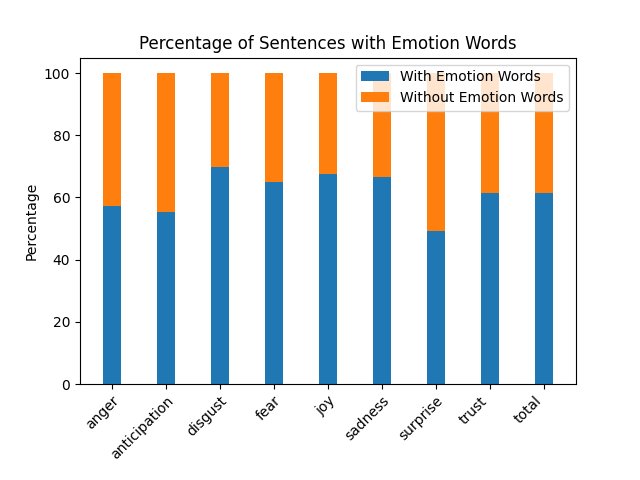
\includegraphics[width=8cm]{./images/emopct.png}
    \caption{Proportion of sentences with emotion intensity values}
    \label{fig:chart}
\end{figure}

Figure 1 shows the percentage of sentences in the dataset contain words with emotion intensity values. About 61.5\% of all sentences in the dataset contain emotion words - this indicates that the lexicon used is limited in what words it perceives as being associated with emotions, and that the use of n-grams as baseline features is necessary in order to obtain sufficient feature data for the rest of the sentences.

\subsection{Classification Model}
This study utilized a linear Support Vector Machine (SVM) classifier using the one-vs-rest strategy for multi-label classification. Implementation was done using the LinearSVC class from scikit-learn. Linear SVM works by using labeled training data to find an optimal hyperplane that can separate classes in a given space\cite{Shalev1}. The one-vs-rest strategy involves splitting a multi-label classification problem into multiple binary classifications\cite{Brownlee1}. A linear SVM was trained for each class, which will learn to distinguish its respective class against all other classes. The LinearSVC classifier was initialized with balanced class weights and a regularization parameter of 0.01, as this resulted in the best classification performance.

\subsection{Model Evaluation}

Two versions of the classifier were created for this study. One classifier features only the baseline features while the other includes the values derived from emotion word intensities. The accuracy of the models were analyzed based on their F1 score, which is calculated as the harmonic mean of the precision and recall of the model, where precision is the fraction of true positives among all predicted positives for a class, and recall is the fraction of true positives among all actual positives for a class. The F1 scores for each of the emotion labels were obtained and compared, as well as the macro F1 score calculated by getting the average of the F1 scores for each label. The most important n-gram and emotion intensity features were also be analyzed by obtaining the coefficients for each linear SVM. In linear SVMs, a feature having a coefficient value closer to 1.0 indicates a strong positive correlation with the given label, while a value closer to -1.0 indicates a strong negative correlation.

\begin{figure}[h!]
    \begin{equation*}
    {Precision_{class} = \frac{TP_{class}}{TP_{class}+FP_{class}}}
    \end{equation*}
    \begin{equation*}
    {Recall_{class} = \frac{TP_{class}}{TP_{class}+FN_{class}}}
    \end{equation*}
    \begin{equation*}
    {F1_{class} = \frac{2 * Precision * Recall}{Precision + Recall}}
    \end{equation*}
    \begin{equation*}
    {F1_{MacroAvg} = \frac{F1_{class1}+F1_{class2}+...+F1_{classX}}{X}}
    \end{equation*}
    \caption{Evaluation Metrics}
\end{figure}

% RESULTS AND DISCUSSION
\section{Results and Discussion}
\subsection{Emotion Intensity}
Each sentence in the dataset was searched for emotion words and the emotion intensity values obtained were added up. Shown in the figure below are the average emotion intensity values for each emotion label.

\begin{figure}[h!]
    \centering
    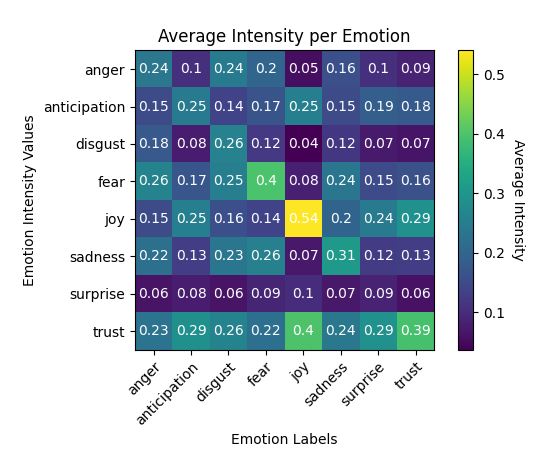
\includegraphics[width=8cm]{./images/avgint2.png}
    \caption{Average emotion intensity values for each emotion label}
    \label{fig:chart}
\end{figure}

Based on Figure 3, it can be observed that certain emotion intensity values have a higher average value across all labels compared to others. Words that express trust and joy appear frequently in sentences regardless of label, while words expressing surprise appear very little across all sentences. For most emotion intensities, the label representing a particular emotions contain the highest intensity value for that emotion across all other labels. Sentences labeled with joy in particular have very high intensity values for joy and low values for negative emotions such as anger, disgust, and sadness. The joy label also has highest average intensity values for trust and surprise across all labels.

\subsection{Evaluation of Classification Model}
The models were evaluated based on their predicted emotion labels compared to the true labels provided in the dataset. As the dataset is multi-labeled, a given sentence may have multiple true labels. If the model were to predict a label which was not part of the true labels, it would count as a false positive for that particular label. Likewise, if the model failed to identify a label that was part of the true labels, it would be counted as a false negative for that label.

\begin{table}[h!]
    \centering
    \emph{Table 6: F1 scores for each label}
    \resizebox{\columnwidth}{!}{%
    \begin{tabular}{|l|l|l|l|}
    \hline
        Class & \begin{tabular}[c]{@{}l@{}}F1 score \\ (with emotion intensities)\end{tabular} & \begin{tabular}[c]{@{}l@{}}F1 score \\ (without emotion intensities)\end{tabular} & Difference \\ \hline
        Anger & 0.4840 & 0.4773 & 0.0067\\ 
        \hline
        Anticipation & 0.4873 & 0.4802 & 0.0071\\ 
        \hline
        Disgust & 0.3854 & 0.3608 & 0.0246\\ 
        \hline
        Fear & 0.4091 & 0.3862 & 0.0229\\ 
        \hline
        Joy & 0.5518 & 0.5224 & 0.0294\\ 
        \hline
        Sadness & 0.4338 & 0.4113 & 0.0225\\ 
        \hline
        Surprise & 0.4148 & 0.3988 & 0.0160\\ 
        \hline
        Trust & 0.4170 & 0.4071 & 0.0099\\ 
        \hline
        Macro Average & 0.4479 & 0.4305 & 0.0174\\
        \hline
    \end{tabular}%
    }
\end{table}

Table 6 shows the F1 scores obtained for each class for both classifiers. The model with emotion intensity features has higher F1 scores for all labels compared to the model without these features, showing that the addition of emotion intensity values can improve classification performance. The disgust, fear, joy, and sadness labels show the most improvement in performance, increasing their F1 scores by more than 0.02.

The 'joy' emotion label achieved the highest F1 score at 0.5518, indicating that the model with emotion intensity values performs well at identifying sentences which express joy. All other labels in the model achieve an F1 score lower than 0.5, resulting in a macro average F1 score of 0.4479 across all labels. This indicates that the classifier has much room for improvement, either in the form of additional feature extraction or through the use of a more advanced classification model.

\subsection{Feature Importance}
The most important features in the model were identified based on their coefficient values in the linear SVMs. A high positive coefficient value indicates a strong positive correlation with the given label, while a high negative coefficient indicates a strong negative correlation with the label. The n-gram and emotion intensity features were then separated to provide a better visualization of the findings.

\begin{table*}
    \centering
    \emph{Table 7: Five highest positive coefficient n-grams for each label (model with emotion intensities)}\\
    \resizebox{18cm}{!}{%
    \begin{tabular}{|ll|ll|ll|ll|ll|ll|ll|ll|}
    \hline
    \multicolumn{2}{|l|}{Anger} & \multicolumn{2}{l|}{Anticipation} & \multicolumn{2}{l|}{Disgust} & \multicolumn{2}{l|}{Fear} & \multicolumn{2}{l|}{Joy} & \multicolumn{2}{l|}{Sadness} & \multicolumn{2}{l|}{Surprise} & \multicolumn{2}{l|}{Trust} \\ 
    \hline
    \multicolumn{1}{|l|}{n-gram} & coefficient & \multicolumn{1}{l|}{n-gram} & coefficient & \multicolumn{1}{l|}{n-gram} & coefficient & \multicolumn{1}{l|}{n-gram} & coefficient & \multicolumn{1}{l|}{n-gram} & coefficient & \multicolumn{1}{l|}{n-gram} & coefficient & \multicolumn{1}{l|}{n-gram} & coefficient & \multicolumn{1}{l|}{n-gram} & coefficient \\ 
    \hline
    \multicolumn{1}{|l|}{'fuck'} & 0.60        & \multicolumn{1}{l|}{'ill'}   & 0.59        & \multicolumn{1}{l|}{'stupid'}   & 0.51        & \multicolumn{1}{l|}{'troubl'} & 0.41        & \multicolumn{1}{l|}{'nice'}  & 0.73        & \multicolumn{1}{l|}{'sorri'} & 0.68        & \multicolumn{1}{l|}{'thought'}   & 0.43        & \multicolumn{1}{l|}{'worri'}      & 0.46        \\ 
    \hline
    \multicolumn{1}{|l|}{'shut'}     & 0.37        & \multicolumn{1}{l|}{'readi'}  & 0.38       & \multicolumn{1}{l|}{'drunk'}      & 0.39       & \multicolumn{1}{l|}{'uh'}     & 0.36        & \multicolumn{1}{l|}{'great'} & 0.59        & \multicolumn{1}{l|}{'poor'}  & 0.58        & \multicolumn{1}{l|}{'dont know'}      & 0.37       & \multicolumn{1}{l|}{'ill'}        & 0.44        \\ 
    \hline
    \multicolumn{1}{|l|}{'stop'}     & 0.36        & \multicolumn{1}{l|}{'tonight'} & 0.36       & \multicolumn{1}{l|}{'bullshit'}    & 0.32        & \multicolumn{1}{l|}{'kill'}   & 0.35        & \multicolumn{1}{l|}{'thank'} & 0.48        & \multicolumn{1}{l|}{'cant'}  & 0.49        & \multicolumn{1}{l|}{'oh'} & 0.35        & \multicolumn{1}{l|}{'thank'}      & 0.39        \\ 
    \hline
    \multicolumn{1}{|l|}{'goddamn'} & 0.35        & \multicolumn{1}{l|}{'let'}  & 0.34       & \multicolumn{1}{l|}{'mother'} & 0.29        & \multicolumn{1}{l|}{'god'}    & 0.33        & \multicolumn{1}{l|}{'fine'}  & 0.46        & \multicolumn{1}{l|}{'never'} & 0.46        & \multicolumn{1}{l|}{'whi'}        & 0.35        & \multicolumn{1}{l|}{'dont worri'} & 0.36        \\ 
    \hline
    \multicolumn{1}{|l|}{'bullshit'} & 0.35        & \multicolumn{1}{l|}{'hell'} & 0.33       & \multicolumn{1}{l|}{'peopl'}   & 0.27        & \multicolumn{1}{l|}{'pleas'}  & 0.33        & \multicolumn{1}{l|}{'love'}  & 0.31       & \multicolumn{1}{l|}{'didnt'} & 0.34        & \multicolumn{1}{l|}{'surpris'}       & 0.35        & \multicolumn{1}{l|}{'help'}       & 0.33       \\ 
    \hline
    \end{tabular}%
    }
\end{table*}

\begin{table*}
    \centering
    \emph{Table 8: Five highest positive coefficient n-grams for each label (model without emotion intensities)}\\
    \resizebox{18cm}{!}{%
    \begin{tabular}{|ll|ll|ll|ll|ll|ll|ll|ll|}
    \hline
    \multicolumn{2}{|l|}{Anger} & \multicolumn{2}{l|}{Anticipation} & \multicolumn{2}{l|}{Disgust} & \multicolumn{2}{l|}{Fear} & \multicolumn{2}{l|}{Joy} & \multicolumn{2}{l|}{Sadness} & \multicolumn{2}{l|}{Surprise} & \multicolumn{2}{l|}{Trust} \\ 
    \hline
    \multicolumn{1}{|l|}{n-gram} & coefficient & \multicolumn{1}{l|}{n-gram} & coefficient & \multicolumn{1}{l|}{n-gram} & coefficient & \multicolumn{1}{l|}{n-gram} & coefficient & \multicolumn{1}{l|}{n-gram} & coefficient & \multicolumn{1}{l|}{n-gram} & coefficient & \multicolumn{1}{l|}{n-gram} & coefficient & \multicolumn{1}{l|}{n-gram} & coefficient \\ 
    \hline
    \multicolumn{1}{|l|}{'fuck'} & 0.62        & \multicolumn{1}{l|}{'readi'}   & 0.46        & \multicolumn{1}{l|}{'stupid'}   & 0.51        & \multicolumn{1}{l|}{'kill'} & 0.55        & \multicolumn{1}{l|}{'love'}  & 0.77        & \multicolumn{1}{l|}{'sorri'} & 0.66        & \multicolumn{1}{l|}{'thought'}   & 0.43        & \multicolumn{1}{l|}{'thank'}      & 0.40        \\ 
    \hline
    \multicolumn{1}{|l|}{'hate'}     & 0.39        & \multicolumn{1}{l|}{'tonight'}  & 0.36       & \multicolumn{1}{l|}{'bastard'}      & 0.47       & \multicolumn{1}{l|}{'danger'}     & 0.50        & \multicolumn{1}{l|}{'nice'} & 0.70        & \multicolumn{1}{l|}{'die'}  & 0.56        & \multicolumn{1}{l|}{'surpris'}      & 0.39       & \multicolumn{1}{l|}{'worri'}        & 0.38        \\ 
    \hline
    \multicolumn{1}{|l|}{'damn'}     & 0.39        & \multicolumn{1}{l|}{'come'} & 0.36       & \multicolumn{1}{l|}{'lie'}    & 0.45        & \multicolumn{1}{l|}{'scare'}   & 0.50        & \multicolumn{1}{l|}{'beauti'} & 0.60        & \multicolumn{1}{l|}{'poor'}  & 0.56        & \multicolumn{1}{l|}{'dont know'} & 0.38        & \multicolumn{1}{l|}{'promis'}      & 0.35        \\ 
    \hline
    \multicolumn{1}{|l|}{'shut'} & 0.38        & \multicolumn{1}{l|}{'let'}  & 0.35       & \multicolumn{1}{l|}{'fool'} & 0.45        & \multicolumn{1}{l|}{'troubl'}    & 0.41        & \multicolumn{1}{l|}{'wonder'}  & 0.59        & \multicolumn{1}{l|}{'cant'} & 0.48        & \multicolumn{1}{l|}{'oh'}        & 0.36        & \multicolumn{1}{l|}{'dont worri'} & 0.32        \\ 
    \hline
    \multicolumn{1}{|l|}{'stop'} & 0.38        & \multicolumn{1}{l|}{'wait'} & 0.35       & \multicolumn{1}{l|}{'shit'}   & 0.42        & \multicolumn{1}{l|}{'afraid'}  & 0.40        & \multicolumn{1}{l|}{'great'}  & 0.59       & \multicolumn{1}{l|}{'cri'} & 0.44        & \multicolumn{1}{l|}{'what'}       & 0.36        & \multicolumn{1}{l|}{'right'}       & 0.32       \\ 
    \hline
    \end{tabular}%
    }
\end{table*}

Table 7 and 8 show the five n-grams with the highest positive coefficient for each label for the two models. It can be observed that certain n-grams with a high coefficient value in the model without emotion intensities do not appear in the table for the model with emotion intensities. These n-grams such as 'scare', 'wonder', and 'die' appear in the emotion lexicon. Words that appear in the emotion lexicon already provide emotion intensity values; as such, their respective unigrams are given a lower coefficient value in the model with emotion intensity values. Table 7 therefore provides insight into words which have a high positive correlation with an emotion label yet have not been included in the used lexicon.

\begin{figure}[h!]
    \centering
    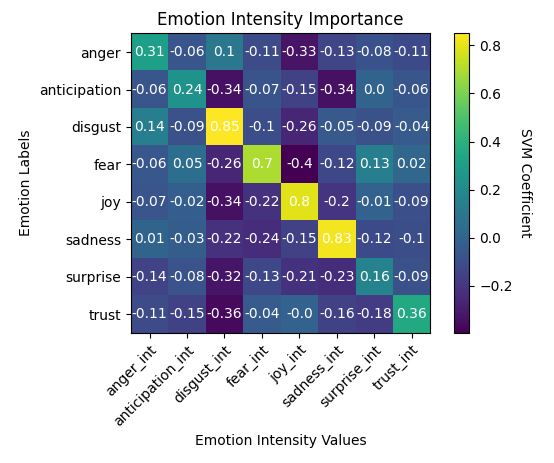
\includegraphics[width=8cm]{./images/emoimp.png}
    \caption{Feature importance for emotion intensity values}
    \label{fig:chart}
\end{figure}

Figure 4 shows the importance of emotion intensity values for each label. Throughout all labels, it can be observed that the the intensity values for the respective emotion label shows the highest importance over the rest of the emotion intensity values. This means that 'anger\_int' is the most important for detecting anger, 'joy\_int' is the most important for detecting joy, and so on. Of note, the intensity values of disgust, fear, joy, and sadness show very high importance for their respective emotion labels, while anger, anticipation, surprise, and trust show relatively less importance. This can be interpreted as a limitation of the lexicon used to obtain the intensity values, as words that may be associated with a given emotion were not indicated as such by the lexicon. For example, several unigrams that show high importance with anger (such as profanities) are not included in the lexicon. Negative correlations can also be observed between emotion intensity values and certain labels, such as joy showing a negative correlation with negative emotion labels such as fear, disgust, and sadness, and vice versa.

\subsection{Statistical Significance}

In order to determine whether the improvements in F1 score observed between the two models are statistically significant, a 10-fold stratified t-test was performed. This was performed with a t-value of 2.262 and a p-value of 0.05. Shown below are the results of the t-test across the F1 scores of the different classes, with the statistically significant classes highlighted in bold:

\begin{table}[h!]
    \centering
    \emph{Table 9: T-statistic and p-value}\\
    \begin{tabular}{|l|l|l|}
        \hline
        F1 score     & t-statistic & p-value        \\ \hline
        \textbf{Macro Average}     & 6.7505      & $8.3601e^{-5}$ \\ \hline
        Anger        & 1.9331      & 0.0852         \\ \hline
        \textbf{Anticipation} & 2.6758      & 0.0254         \\ \hline
        \textbf{Disgust}      & 4.1034      & 0.0027         \\ \hline
        \textbf{Fear}         & 3.0154      & 0.0146         \\ \hline
        \textbf{Joy}          & 4.1379      & 0.0025         \\ \hline
        \textbf{Sadness}      & 4.0615      & 0.0028         \\ \hline
        \textbf{Surprise}     & 2.7542      & 0.0223         \\ \hline
        Trust        & 2.2045      & 0.0549         \\ \hline
    \end{tabular}%
\end{table}

The results of the t-test show that every F1 score has a positive t-statistic, indicating that the F1 score of every class improved when emotion intensity values were added as features for the model. However, the anger and trust classes have t-statistics and p-values that do not meet the defined thresholds, suggesting that the improvement in performance observed in these classes is not statistically significant. The rest of the classes - namely anticipation, disgust, fear, joy, sadness, and surprise, as well as the macro F1 score, are shown to be statistically significant.

% CONCLUSION
\section{Conclusion}
The goal of this study was to use emotion word intensities to identify the presence of one or more emotions within a body of text. The results show that the addition of emotion intensities was able to improve the classification performance of the Linear SVM model. In particular, emotion intensity values for disgust, fear, joy, and sadness showed high feature importance for their respective classes, which was reflected in a larger improvement in F1 score. Certain classes also were able to express a negative correlation with several intensity values, such as with the 'joy' label showing a negative correlation with emotion intensity values of fear and disgust.

Based on the classification results of the model, there is still much room for improvement in regards to the identification of multiple emotions in a body of text. A possible area for improvement for future studies would be to expand upon how emotion intensity values are obtained. The use of an emotion intensity lexicon is ultimately limited by what words are included in it. Only 61.5\% of the sentences in the dataset included emotion intensity, and so the remaining sentences were only able to be classified based on the presence of certain n-grams. Included in the results is a table of words which show high positive correlations with a given emotion label, but were not included in the utilized lexicon. Future studies may take these results into account when considering a lexicon-based approach. Grammar-based modifiers may also be accounted for in the future, as adjectives and negative words can influence the intensity values derived from emotion words. Lastly, future studies may also explore how emojis, special characters, and other figures of speech can influence the emotions expressed by text.

% ACKNOWLEDGMENT
\section*{Acknowledgment}
I would like to thank my adviser, Maria Art Antonette D. Clariño, as her expertise and guidance was crucial through every part of this study. I would also like to thank all my friends and family for supporting my current and future endeavors.

% BIBLIOGRAPHY
\bibliographystyle{IEEE/IEEEtran}
\bibliography{enrique-cs190-ieee}
% \nocite{*}

% BIOGRAPHY
\begin{biography}[{
\includegraphics{enrique.eps}}]{Andrei Francis U. Enrique}
is a BS Computer Science student from the University of the Philippines Los Baños, residing in Mandaluyong City. He has a keen interest in understanding how systems work, especially in the context of software and video game mechanics.
\end{biography}


\end{document}
 
